\setchapterpreamble[u]{\margintoc}
\chapter{Proprietà magnetiche}
\labch{cap5}

Le proprietà magnetiche riguardano solo una particolare classe di materiali metallici, caratterizzati dalla presenza di \textbf{orbitali interni incompleti}: essi prendono il nome di \textbf{metalli di transizione}. Solo i gas nobili hanno gli orbitali completi, ma di solito quelli incompleti sono quelli esterni, che permettono i legami chimici.

Il ferro ha numero atomico 26 e la seguente struttura elettrica: 
\begin{equation*}
    \mathrm{1s^2\, 2s^2\, 2p^6\, 3s^2\, 3p^6\, 4s^2\, 3d^6}.
\end{equation*}
Si nota che l’orditale d è incompleto.
Gli elettroni di conduzione, cioè di valenza, sono quelli nell’orbitale 4s, che costituisce la banda di conduzione: essi possono lasciare il metallo e costituire la nube elettronica.
Le proprietà magnetiche risiedono nell’orbitale 3d: gli elettroni di tale orbitale sono fissi e rimangono legati all’atomo.

Per distinguere i materiali in base alle loro proprietà magnetiche, bisogna analizzare il loro comportamento quando sono sottoposti all’azione di un campo magnetico esterno. Possono verificarsi tre situazioni diverse:
\begin{enumerate}\index{ferromagnetismo}\index{paramagnetismo}\index{diamagnetismo}
    \item il materiale si oppone al campo magnetico esterno: si ha una reazione negativa da parte del materiale e una rarefazione del campo magnetico $\to$ \textbf{diamagnetismo}. Gli elettroni si muovono nell’atomo cercando di annullare le cariche per raggiungere la minima energia possibile. La presenza del campo magnetico esterno disturba il moto degli elettroni: essi cominceranno a ruotare in modo distorto, creando un campo magnetico interno che si oppone imposto dall’esterno;
    \item il materiale rafforza notevolmente il campo magnetico esterno: si ha una reazione positiva da parte del materiale e un rafforzamento del campo magnetico $\to$ \textbf{ferromagnetismo};
    \item il materiale rafforza debolmente il campo magnetico esterno $\to$ \textbf{paramagnetismo}.
\end{enumerate}

\begin{marginfigure}[3cm]
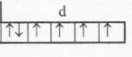
\includegraphics{images/img20.png}
\caption{Occupazione dell'orbitale 3d del ferro }
\labfig{img20}
\end{marginfigure}
Nel caso del ferro, l’orbitale d potrebbe contenere 10 elettroni, ma ne contiene solo 6. Essi sono disposti in modo da occupare tutti gli orbitali, secondo il principio di
minima energia (massima entropia) e il principio di esclusione\index{principio di esclusione} di Pauli (regola di Huns): avremo un orbitale con due elettroni e 4 con un solo elettrone.
Avendo quattro elettroni spaiati, senza il rispettivo antagonista: essi ruotando creano un momento magnetico elementare residuo. Nella
realtà, a causa dei fenomeni di schermaggio, si creano 2,6 momenti magnetici residui, invece che 4 per ogni singolo atomo.
All’interno del ferro vi è una struttura ordinata in domini magnetici o \textbf{domini di Weiss}\index{domini di Weiss}, cioè zone caratterizzate dall’iso-orientamento dei momenti magnetici residui di tutti gli atomi presenti nel singolo dominio. Tutti i domini hanno diversi orientamenti e quindi, esternamente il materiale non ha effetti magnetici, cioè non è una calamita.
Immergendo il materiale in un campo magnetico esterno, progressivamente tutti i domini tendono a orientarsi nella stessa direzione e verso del campo magnetico esterno, rafforzandolo. Si ha dunque una situazione di iso-orientamento dei momenti magnetici residui in tutto il materiale, che caratterizza il fenomeno del ferromagnetismo.
Si raggiunge la condizione di saturazione, quando tutti i domini sono ido-orientati: la curva B-H presenta, infatti, un asintoto (vedi \reffig{img21}).
\begin{figure}[hb]
    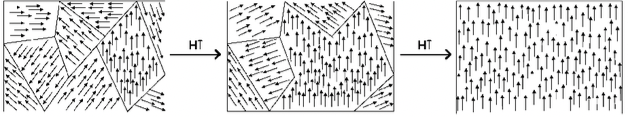
\includegraphics[width=1\textwidth]{images/img21.png}
    \caption{Evoluzione dei domini di Weiss per effetto di un campo magnetico H, rivolto verso l'alto}
    \labfig{img21}
\end{figure}

Giunti alla saturazione, rimuovendo il campo magnetico esterno, verificare due situazioni:
\begin{itemize}
    \item il materiale ritorna alle condizioni iniziali, con la disorientazione dei domini, in modo reversibile: si parla, allora, di \textbf{materiali magneticamente dolci}. Il materiali ritorna nella sua condizione di energia minima. Se il materiale non ha difficoltà a deformarsi, cioè non oppone resistenza allo scorrimento delle dislocazioni (poco carbonio, grossi cristalli di ferro, pochi bordi di grano), si tratta di un materiale dolce, in cui i domini possono facilmente ritornare alle condizioni iniziali, riarrangiandosi. In questo caso si ottiene una \textbf{elettrocalamita}: sotto l’azione del campo magnetico il materiale diventa una calamita; una volta tolto il campo magnetico, esso diventa nuovamente inerte. I materiali dolci sono costituiti da ferro pressoché puro, in quanto il carbonio rimasto nel ferro si oppone al moto dislocativo. Si utilizzano, quindi, lamierini per trasformatori costituiti da acciai al silicio: mettendo il 4-5\% di silicio, il carbonio abbandona il reticolo dell’acciaio e le dislocazioni si muovono molto più facilmente. Il silicio, infatti, è un atomo sostituzionale, che interferisce solo con le dislocazioni a spigolo, e non interstiziale come il carbonio, che interferisce con le dislocazioni a vite e a spigolo.
    \item fenomeno dell’\textbf{isteresi}: una volta annullato il campo magnetico, il materiale rimane magnetizzato e per annullare il campo magnetico residuo bisognerà quindi applicare un campo magnetico in verso opposto. I domini del materiale rimangono orientati: si è creata una calamita. Questo comportamento è tipico dei \textbf{materiali magneticamente duri}, costituiti da cristalli fini, elementi leganti e un alto tenore di carbonio, che disturbano il movimento delle dislocazioni. Le calamite sono molto fragili, in quanto le dislocazioni non hanno possibilità di muoversi.
\end{itemize}
\index{curve di isteresi}
\begin{marginfigure}[-9cm]
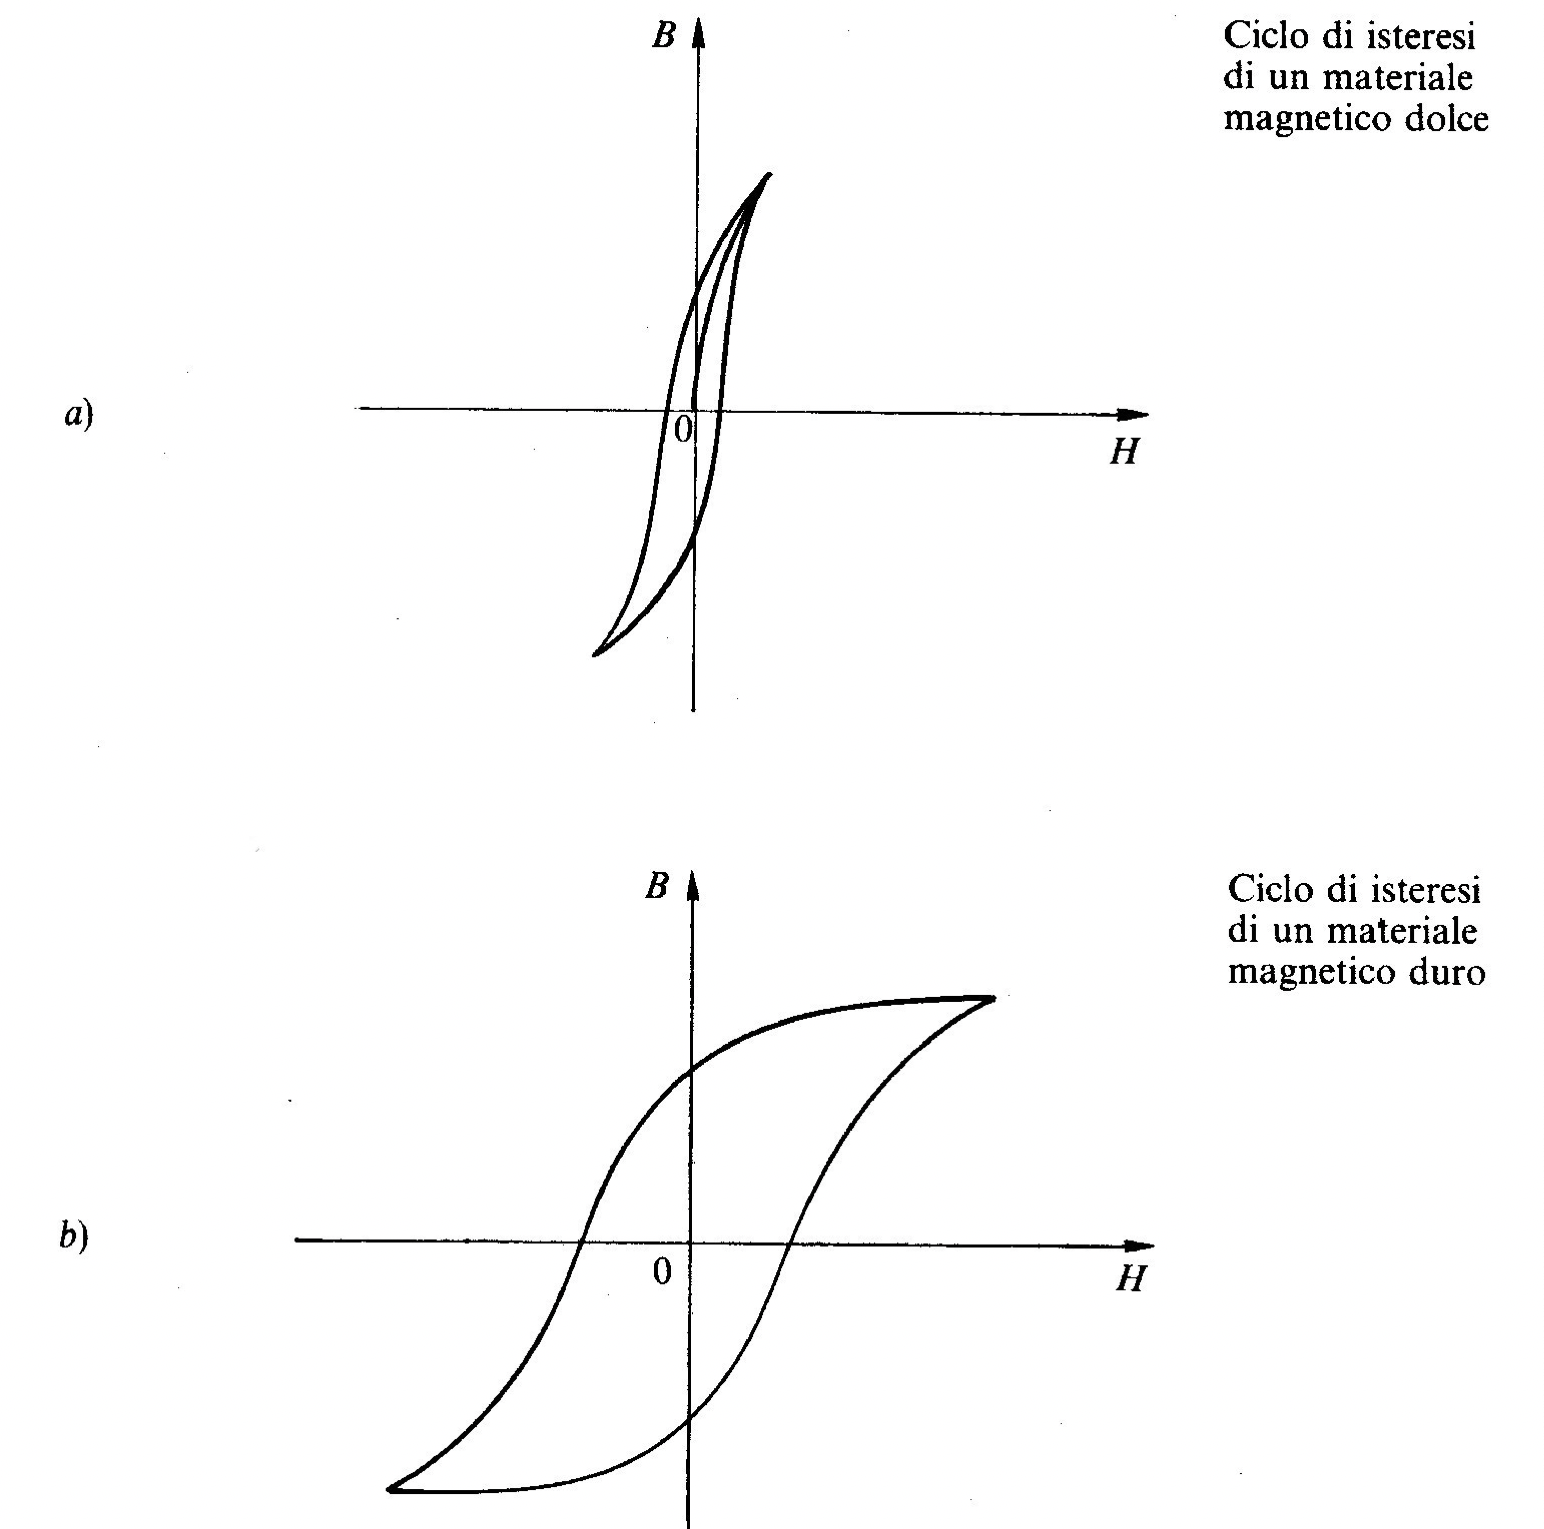
\includegraphics{images/img22.png}
\caption{Curve di isteresi per materiali magnetici dolci (in alto) e duri (in basso) a confronto}
\end{marginfigure}

Fino ad ora si è ragionato a temperatura ambienti, ma cosa succede variando la \textbf{temperatura}?

 Se si raggiunge la \textbf{temperatura di Curie}\index{temperatura di Curie}, il materiale da ferromagnetico diventa paramagnetico.
E’ importante quindi che il materiale sia ferromagnetico a temperature industrialmente apprezzabili. Solo tre elementi hanno questa proprietà: il ferro (768°C), il cobalto (1115°C) e il nichel a (353°C). Quando un materiale viene scaldato fino al raggiungimento della temperatura di Curie, l’entropia diventa il fattore determinante: aumentano il disordine, i domini vengono distrutti e si annulla l’iso-orientamento al loro interno, facendo diventare il materiale paramagnetico.

Un altro comportamento magnetico è quello del ferrimagnetismo, che è una disposizione nella quale i domini non sono tutti iso-orientati, ma la risultante dei momenti magnetici residui è comunque diversa da zero, in una certa direzione.

La magnetoscopia permette di verificare se il ferro è autentico o ferritico, anche solo utilizzando una calamita: essa non si attacca nel primo caso, mentre si attacca nel secondo\sidenote{I sottomarini vengono costruiti in acciaio INOX austenitico, in modo da non attrarre bombe di profondità magnetiche. Il lettore più attento si renderà conto che fare le eliche dei motori con questo materiale porterebbe a problemi di resistenza a fatica, e avrebbe proprio ragione. Vengono in genere costruiti con INOX ferritici e schermati successivamente con qualche altro metodo}.